\section{Preliminaries}
\label{sec:perliminary}

\begin{figure}[tbp]
	\hspace{0ex}
	\vspace{0ex}
	\centering
	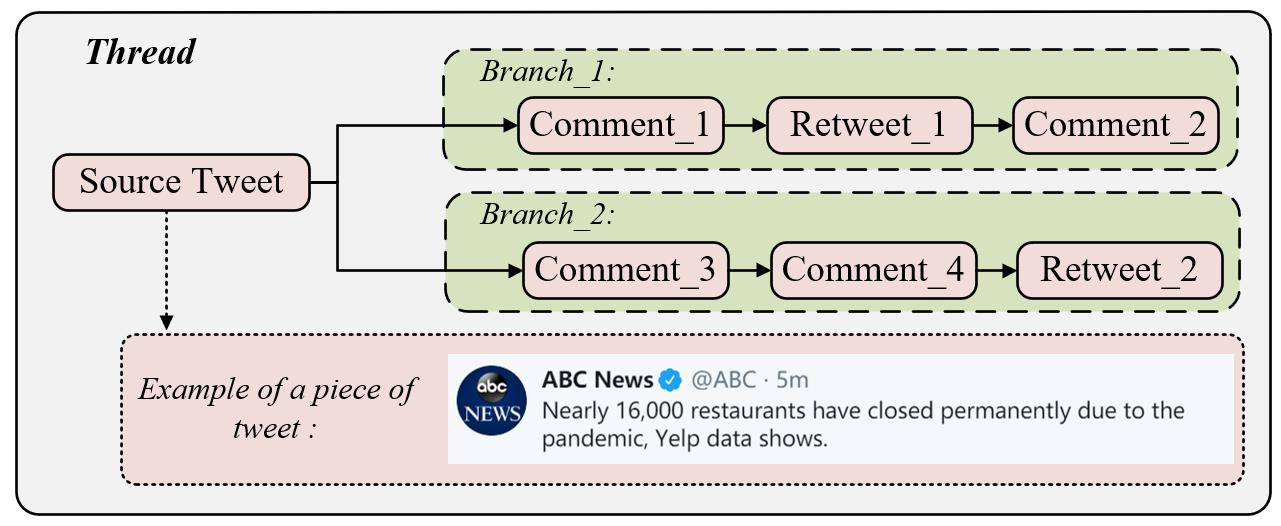
\includegraphics[width = \textwidth]{fig/data_format}
	\caption{The data format of a tweet thread}
	\label{fig:data_format}
\end{figure}

In this section, we proceed to introduce the notations, problem definitions, and background knowledge of rumor tracking. The frequently used notations are summarized in Table.~\ref{tab:notations}.

\subsection{Social Network Data}
\label{sec:social_network_data}
We use two benchmark datasets PHEME\cite{DBLP:conf/coling/KochkinaLZ18} and RumorEval\cite{DBLP:conf/semeval/EnayetE17}. These datasets contain several rumor events and each event consists of numerous tweet threads. The data format of a tweet thread is shown in Fig.~\ref{fig:data_format}. As shown, a tweet thread is a tree structure. The root node corresponds to a source tweet and the branches correspond to a tweet sequence that includes retweets and comments. A tweet contains various types of features, including content, publication time, screen name, etc. The statistical details of PHEME and RumorEval are shown in Table \ref{tab:pheme} and Table \ref{tab:RumorEval}, respectively.

\begin{table}
	\caption{Notation Summarization}
	\centering
	\label{tab:notations}
	\begin{tabular}{|c|l|}
		\hline
		\textbf{Notation} & \textbf{Definition}\\
		\hline
		$T$ & the set of tweets \\
		\hline
		$y_F'$ & output of FastText \\
		\hline
		$t_n$ & a tweet\\
		\hline		
		$y_T'$ & output of TextCNN\\
		\hline
		$C$ & the set of rumor events\\
		\hline
		$y_B'$ & output of BiLSTM\\
		\hline
		$c_m$ & a rumor event \\
		\hline
		$y_N'$ & output of Naive Bayes\\
		\hline
		$r$ & predictable result of a component\\
		\hline
		$y_S'$ & output of SGD\\
		\hline
		$R$ & predictable result of ART\\
		\hline
		$y'$& output of the ART\\
		\hline
		$x \in R^{l*d}$ & a processed sample\\
		\hline
		$y \in R^m$ & a training label\\
		\hline
		$K_y$ & set of all components outputs\\		
		\hline						
	\end{tabular}
\end{table}

\subsection{Problem Definition}
\label{sec:problem}
Let $T = \left\{t_1, t_2, ..., t_n \right\}$ denote the set of tweets and each tweet is denoted as $t_n$. Let $C = \left\{c_1, c_2, ... , c_m \right\}$ denote the set of rumor events and $c_m$ denotes a particular rumor event. Each tweet is assigned to only one rumor event. For each given tweet $t_n$, the goal of rumor tracking is to find the most relevant rumor event. In this work, we transform the binary rumor tracking problem (relevant/irrelevant) into an m-way classification problem. 

We conduct a preprocessing procedure to embed the $T$ and $C$ into vectors. In preprocessing, a tweet $t_n \in T $ is padded to a fixed length $l$. Then, each word in the l-length tweet $t_n$ is embedded to a d-dimensional vector so that the $t_n$ is transformed to an tensor $x^{(i)} \in R^{l*d}$. Also, we embed each event $c_m \in C$ to a one-hot vector $y^{(i)} \in R^m$. By preprocessing, the dataset is transformed into: $$\left\{ (x^{(1)}, y^{(1)}), (x^{(2)}, y^{(2)}),..., (x^{(n)}, y^{(n)}) \right\}, x^{(i)} \in R^{l*d}, y^{(i)} \in R^m $$ The goal is transformed to predicting the $y^{(i)}$ for a given $x^{(i)}$. Also, for a testing sample $x^{(i)}$, we set the branch or thread that it belongs to is unknown in advance. 

In a rumor event, source tweets are collected by keywords, and therefore the source tweets are highly similar to each other. We find that the similarity of source tweet disturbs the classification of tweets. To verify our assumption, we conduct an experiment to train a rumor event classifier with source tweets as inputs. The classification result suggests that the accuracy reaches even 100\%. Consequently, we cut down the link between tweet and its source, and then process each tweet independently to get a convincing result. 

\subsection{Basic Models for Text Classification}
\label{sec:deeplearning_model} 
In this section, we proceed to introduce some basic text classification models that are the components of ART.

\subsubsection{Machine Learning based Models}
\textbf{Naive Bayes} \cite{DBLP:journals/ml/DomingosP97} assumes that all input variables are independent of each other. By multiplication the conditional probability, it achieves classification task with small quantities of parameters. Naive Bayes model is widely adopted in the short text classification problem, showing a pretty good performance. The procedure of Naive Bayes is denoted as following:
\begin{align}\label{eq:nb}
y_{N_{i}}' &= \frac{P(y_i)\prod_{j = 0}^d P(x_j|y_i)}{\prod_{j = 0}^d P(x_j)},\\
y_N' &= concat(y_{N_{1}}',y_{N_{2}}',..., y_{N_{i}}'),
\end{align}
where $x_j$ is a component of $x$, corresponding to a word in tweet.  $y_i$ is a component of training sample $y$. $y_{N_{i}}'$ is a component of $y_N'$, representing the probability of a classification. We choose Naive Bayes as  a component of the ART and  $y_N'$ is the final output of it.

\textbf{SGD} \cite{avriel2003nonlinear} is a parameter update policy in machine learning, which updates parameters for each single sample. SGD based machine learning models are trained on large scale datasets by incremental learning. We denote the procedure of SGD based model as $S()$, and the output of SGD components is:
\begin{equation}\label{eq:sgd}
y_S' = S(TFIDF(x)),
\end{equation}
where TFIDF is Term Frequency-Inverse Document Frequency. Finally, we choose the SGD based classification model as the component of the ART, and $y_S'$ denotes its output.

\subsubsection{Deep Learning based Models}

\textbf{FastText} \cite{DBLP:journals/tacl/BojanowskiGJM17, DBLP:journals/corr/JoulinGBDJM16, DBLP:conf/eacl/GraveMJB17} is an extension of the skip-gram model introduced by Mikolov et al. \cite{DBLP:conf/nips/MikolovSCCD13}. The main difference between FastText and skip-gram is that the predictable target of FastText is a classification label rather than a middle word. Also, FastText adopts hierarchical softmax to deal with the large corpus and vocabulary dictionary. With the help of these optimizations, FastText classifies large amounts of texts in a short time. We choose the FastText as a component of the ART and denote its output as $y_F'$.

\textbf{BiLSTM} \cite{DBLP:journals/neco/HochreiterS97} is Bi-directional Long Short-Term Memory, which is consisted of a forward-LSTM and a backward-LSTM. BiLSTM effectively learns the long term dependency of sequential data. So we usually treat it as a evolution of LSTM and it is suitable for text data. The details of BiLSTM are following:
\begin{align}\label{eq:lstm}
x_tL/R &= Embedding(x_tL/R), \\
x_t &= concat(x_tL, x_tR), \\
i_t &= \sigma(W_i \cdot [h_{t-1}, x_t] + b_i),\\
f_t &= \sigma(W_f \cdot [h_{t-1}, x_t]),\\
\widetilde{C_t} &= tanh(W_{\tilde{C_t}} \cdot [r_t C_{t-1}, x_t]  + b_C),\\
C_t &= (1-f_t) C_{t-1} + f_t \widetilde{C_t},\\
h_t &=o_t \* \tanh(C_t),\\
y_B^{'} &= o_t =  \sigma(W_o \cdot h_t),
\end{align}
where $x_t$ is the input at time step $t$, and it is concatenated by leftward unit $x_tL$ and rightward unit $x_tR$. BiLSTM consists of three gates: forget gate $f_t$, input gate $i_t$, and output gate $o_t$. Also, it has two memories: long-term memory $C_t$ and short-memory $h_t$. Finally, we use output $o_t$ as the final output of BiLSTM, denoted as $y_B^{'}$.

\textbf{TextCNN} \cite{DBLP:conf/emnlp/Kim14} uses multiple convolutional filters with different sizes to capture N-gram features. Compared to RNN based models, TextCNN reaches convergence faster due to the parallel computation. The tweets are usually short text (within 140 words) with sparse semantic. Consequently, CNN based models are more suitable than RNN based models for tweets classification where tweets are usually treated as a bag of words. We choose the TextCNN as one of the components of the ART. The brief procedure of TextCNN is shown as follows,

\begin{align}\label{eq:tcnn}
V_x &= Embedding(x), \\
m_3 &= maxpooling(ConV_3(V_x)),\\
m_4 &= maxpooling(ConV_4(V_x)),\\
m_5 &= maxpooling(ConV_5(V_x)),\\
y_T' &= flatten(concat(m_3, m_4, m_5)),
\end{align}
where the $Embedding()$ is the embedding layer, and $m$ is the output of different convolutional filters. By concatenating and flattening, the final output of TextCNN component is denoted as $y_T'$.